\documentclass{article}

\usepackage{graphicx}
\usepackage{amsfonts}
\usepackage{pdfpages}
\usepackage{bbm}
\usepackage{amssymb}
\usepackage[margin=1in]{geometry}
\usepackage{amsmath}
\usepackage{mathtools}

\title{ STAT 321: Assignment 5}
\author{Saksham Sudershan}
\date{26 March 2022}

\begin{document}
\maketitle

\section*{Problem 1}
	\subsection*{(a)}
	Let $\Theta = 1$ denote the case in which Alice is given the first coin whose probability of heads, $p_H=0.3$. Similarly, let $\Theta = 2$ and $\Theta = 3$ denote the case of Alice being given coin 2 and 3 respectively. \hfill \hfill \linebreak Let $X=1$ denote the case in which she gets heads on the first flip, and tails on the second one. 

	$$ \hat\Theta_{MAP} (x) = \arg \max_\theta P(\theta|x)  $$
	
	If Alice was given coin 1, $$ P(\Theta =1|X=1) = \frac{P(\Theta = 1) \cdot P(X=1| \Theta =1 )}{P(\Theta = 1) \cdot P(X=1| \Theta =1 )+P(\Theta = 2) \cdot P(X=1| \Theta =2 )+P(\Theta = 3) \cdot P(X=1| \Theta =3 )}$$
	$$ \Rightarrow P(\Theta = 1|X=1) = \frac{\frac{1}{3} \cdot (0.3 \times 0.7)}{\frac{1}{3} \cdot (0.3 \times 0.7)+\frac{1}{3} \cdot (0.7 \times 0.3)+\frac{1}{3} \cdot (0.5 \times 0.5)} $$
	$$ \Rightarrow P(\Theta = 1|X=1) = \frac{0.07}{0.07+0.07+0.0833} $$
	$$ \therefore P(\Theta = 1|X=1) = 0.3135 $$


	If Alice was given coin 2, $$ P(\Theta =2|X=1) = \frac{P(\Theta = 1) \cdot P(X=1| \Theta =1 )}{P(\Theta = 1) \cdot P(X=1| \Theta =1 )+P(\Theta = 2) \cdot P(X=1| \Theta =2 )+P(\Theta = 3) \cdot P(X=1| \Theta =3 )}$$
	$$ \Rightarrow P(\Theta = 2|X=1) = \frac{\frac{1}{3} \cdot (0.7 \times 0.3)}{\frac{1}{3} \cdot (0.3 \times 0.7)+\frac{1}{3} \cdot (0.7 \times 0.3)+\frac{1}{3} \cdot (0.5 \times 0.5)} $$
	$$ \Rightarrow P(\Theta = 2|X=1) = \frac{0.07}{0.07+0.07+0.0833} $$
	$$ \therefore P(\Theta = 2|X=1) = 0.3135 $$

	If Alice was given coin 3, $$ P(\Theta =3|X=1) = \frac{P(\Theta = 1) \cdot P(X=1| \Theta =1 )}{P(\Theta = 1) \cdot P(X=1| \Theta =1 )+P(\Theta = 2) \cdot P(X=1| \Theta =2 )+P(\Theta = 3) \cdot P(X=1| \Theta =3 )}$$
	$$ \Rightarrow P(\Theta = 3|X=1) = \frac{\frac{1}{3} \cdot (0.5 \times 0.5)}{\frac{1}{3} \cdot (0.3 \times 0.7)+\frac{1}{3} \cdot (0.7 \times 0.3)+\frac{1}{3} \cdot (0.5 \times 0.5)} $$
	$$ \Rightarrow P(\Theta = 3|X=1) = \frac{0.0833}{0.07+0.07+0.0833} $$
	$$ \therefore P(\Theta = 3|X=1) = 0.3730 $$
\linebreak
	Since $P(\theta|x)$ is maximzed for the case that Alice was given coin 1,
	$$ \therefore \hat\Theta_{MAP} (X=1) = 3 $$

	\subsection*{(b)}
	Now, $P(\Theta=1) = 0.6$, $P(\Theta = 2) = 0.4 $ and $P(\Theta =3) = 0$. \hfill \hfill \linebreak
	She only flips the coin once. Let $X=1$ denote the case in which she flips a heads and $X=0$ denote the case in which she flips a tails. \hfill \hfill \linebreak
	
	If Alice flips heads,
	$$ P(\Theta =1|X=1) = \frac{P(\Theta = 1) \cdot P(X=1| \Theta =1 )}{P(\Theta = 1) \cdot P(X=1| \Theta =1 )+P(\Theta = 2) \cdot P(X=1| \Theta =2 )+P(\Theta = 3) \cdot P(X=1| \Theta =3 )}$$
	$$ \Rightarrow P(\Theta = 1|X=1) = \frac{0.6 \cdot 0.3}{0.6 \cdot 0.3+0.4 \cdot 0.7+0 \cdot 0.5} $$
	$$ \Rightarrow P(\Theta = 1|X=1) = \frac{0.18}{0.18+0.28+0} $$
	$$ \therefore P(\Theta = 1|X=1) \approx 0.4737 $$
	
	$$  P(\Theta =2|X=1)  = \frac{0.28}{0.18+0.28} $$
	$$ \therefore  P(\Theta =2|X=1)  \approx 0.7368 $$ 

	And, $$ P(\Theta =3|X=1)  = 0 $$
\linebreak

	If Alice flips tails,
	$$ P(\Theta =1|X=0) = \frac{P(\Theta = 1) \cdot P(X=0| \Theta =1 )}{P(\Theta = 1) \cdot P(X=0| \Theta =1 )+P(\Theta = 2) \cdot P(X=0| \Theta =2 )+P(\Theta = 3) \cdot P(X=0| \Theta =3 )}$$
	$$ \Rightarrow P(\Theta = 1|X=0) = \frac{0.6 \cdot 0.7}{0.6 \cdot 0.7+0.4 \cdot 0.3+0 \cdot 0.5} $$
	$$ \Rightarrow P(\Theta = 1|X=0) = \frac{0.42}{0.42+0.18+0} $$
	$$ \therefore P(\Theta = 1|X=0) \approx 0.8 $$
	
	$$  P(\Theta =2|X=0)  = \frac{0.12}{0.42+0.12} $$
	$$ \therefore  P(\Theta =2|X=0)  = 0.2 $$ 

	And, $$ P(\Theta =3|X=0)  = 0 $$
\linebreak

	Thus, $\hat\Theta_{MAP} (X=1) = 2 $ and $\hat\Theta_{MAP} (X=0) = 1$. \hfill \hfill \linebreak

	Now, the overall probability of error is given by,
	$$ P(\hat\Theta_{MAP} \neq \Theta) = P(\Theta = 1, X = 1) + P(\Theta = 3, X = 1) +P(\Theta = 2, X=0)+P(\Theta = 3, X = 0)  $$
	$$ \therefore P(\hat\Theta_{MAP} \neq \Theta) = 0.4737 + 0+0.2+0 = 0.6737 $$

\section*{Problem 2}
\subsection*{(a)}
	We know the radioactivity level of "Iocane" has the $Unif[0,1]$ distribution, and that of "Sennari" has the $Exp(1)$ distribution. \hfill \hfill \linebreak
	Let $\Theta = 1$ denote that the bottle has "Iocane" and $\Theta = 2$ denote that the bottle has "Sennari". \hfill \hfill \linebreak
	Let $X=x$ denote radioactivity measured. \hfill \hfill \linebreak
	We know that,
	$$ \hat\Theta_{MAP} = \arg \max_\theta \; P(\theta | x) $$
	If the bottle contains "Iocane",
	$$ P(\Theta = 1 | X = x) = \frac{P(\Theta = 1) \cdot P(X=x|\Theta = 1)}{P(\Theta = 1) \cdot P(X=x|\Theta = 1)+P(\Theta = 2) \cdot P(X=x|\Theta = 2)}$$
	$$ P(\Theta = 1 | X = x) =  \begin{dcases}
		\frac{\frac{1}{2}\cdot \frac{1}{1-0}}{\frac{1}{2}\cdot \frac{1}{1-0}+\frac{1}{2}\cdot e^{-x}} & 0 \leq x \leq 1 \\
		0 & x >1 
		\end{dcases}
	$$
	$$ \therefore P(\Theta = 1 | X = x) =  \begin{dcases}
		\frac{1}{1+e^{-x}} & 0 \leq x \leq 1 \\
		0 &  x > 1
		\end{dcases}
	$$
\linebreak
	If the bottle contains "Sennari",
	$$ P(\Theta = 2 | X = x) = \frac{P(\Theta = 2) \cdot P(X=x|\Theta = 2)}{P(\Theta = 1) \cdot P(X=x|\Theta = 1)+P(\Theta = 2) \cdot P(X=x|\Theta = 2)}$$
	$$ P(\Theta = 2 | X = x) =  \begin{dcases}
		\frac{\frac{1}{2}\cdot e^{-x}}{\frac{1}{2}\cdot \frac{1}{1-0}+\frac{1}{2}\cdot e^{-x}} & 0 \leq x \leq 1 \\
		1 & x >1 
		\end{dcases}
	$$
	$$ \therefore P(\Theta = 2 | X = x) =  \begin{dcases}
		\frac{e^{-x}}{1+e^{-x}} & 0 \leq x \leq 1 \\
		1 &  x > 1
		\end{dcases}
	$$
	We know that,
	$$ \frac{e^{-x}}{1+e^{-x}} \ is\ a\ monotonically\ increasing\ function. $$
	At $x=0$, $ P(\Theta = 1 | X = x)  = 0.5$. And at $x=1$, $ P(\Theta = 1 | X = x) = 0.731 $. Thus, when $x=0$, we can choose "Iocane" or "Sennari" arbitrarily; and at any point $0<x\leq 1$, $ \hat\Theta_{MAP}=1$, or we choose "Iocane".
\linebreak

	Thus our decision rule is dependent upon our measure of radioactivity of the bottle. 
	$$ \Rightarrow \hat\Theta_{MAP} = \begin{dcases}
		1\ or\ 2\ (chosen\ arbitrarily) & x = 0 \\
		1 & 0 < x \leq 1 \\
		2 & x>1
		\end{dcases}
	$$

\subsection*{(b)}
	Let's assume we choose "Iocane" always at $x=0$. Thus, our probability of error is given by,
	$$ P(\hat\Theta_{MAP} \neq \Theta) = P(\Theta=2, x=0) + P(\Theta =2, 0<x\leq 1) + P(\Theta = 1, x>1) $$
	Or,
	$$ \begin{aligned}
		P(\hat\Theta_{MAP} \neq \Theta) & = P(\Theta =2, 0\leq x\leq 1) + P(\Theta = 1, x>1) &  \\
		 & = P(\Theta = 2) \times P(0 \leq x \leq 1 | \Theta =2 ) + P(\Theta = 1) \times P(x> 1 | \Theta =1 ) & \\
		& = \frac{1}{2} \cdot [1-e^{-1}] + \frac{1}{2}\cdot 0 & Using\ CDF\ of\ Exp(1)\ distribution\ \\
		& = \frac{1}{2} \cdot 0.6321 \\
		& = 0.316 
		\end{aligned}
	$$  
\linebreak

	So the associated probability of error for our decision rule is $0.316$.

\section*{Problem 3}
	We know that,
	$$ S = \begin{dcases}
		-1 & with\ probability\ \frac{1}{3} \\
		0 & with\ probability\ \frac{1}{3} \\
		1 & with\ probability\ \frac{1}{3}
		\end{dcases}
	$$
	$$ f_Z (z) = \frac{\lambda}{2} e^{-\lambda |z|} $$
	And, $$ Y = S + Z $$
	$$ \Rightarrow Z = Y - S $$

\subsection*{(a)}
	We have to find $f_{Y|S} (y|s)$ for $s= -1, 0, 1$. \hfill \hfill \linebreak
	
	Let $s=-1$.
	$$ \begin{aligned}
		f_{Y|S} (y|s) &= f_{Z|S} (y-s|s) \; \; & Since\ Z = Y-S \\
				&= f_{Z} (y-s) & Since\ Z\ and\ S\ are\ independent\ \\
				&= f_Z (y+1) & \\
				&=\frac{\lambda}{2} e^{-\lambda |y+1|} & 
		\end{aligned} $$
\linebreak
	
	Let $s=0$. Similarly,
	$$ \begin{aligned}
		f_{Y|S} (y|s) &= f_Z (y) \\
				&=\frac{\lambda}{2} e^{-\lambda |y|} & 
		\end{aligned} $$
\linebreak

	And let $s=-1$. Again,
	$$ \begin{aligned}
		f_{Y|S} (y|s) &= f_Z (y-1) & \\
				&=\frac{\lambda}{2} e^{-\lambda |y-1|} & 
		\end{aligned} $$

\subsection*{(b)}
	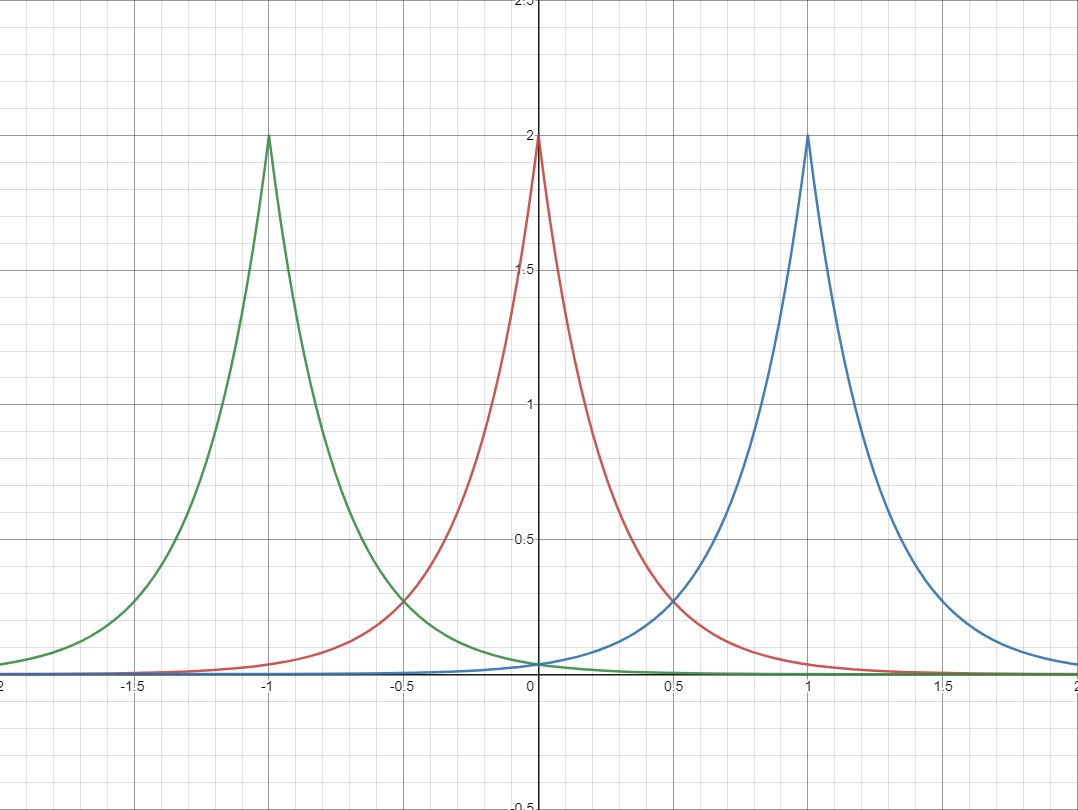
\includegraphics[width=\textwidth]{plot1}
	We can find the critical points for when $\hat{S}_{MAP} (y)$ changes for given value of $y$ by equating:
	$$ f_Z (y+1) = f_Z (y) \; \; \; \; \; \; \; when\ y \in (-1,0) $$
	$$ \Rightarrow \frac{\lambda}{2} e^{-\lambda |y+1|} = \frac{\lambda}{2} e^{-\lambda |y|} $$
	$$ \Rightarrow |y+1| = |y| $$
	$$ \Rightarrow y+1 = -y $$
	$$ \therefore y= -0.5 $$

	And, $$ f_Z (y) = f_Z (y-1) \; \; \; \; \; \; \; when\ y \in (0,1) $$
	$$ \Rightarrow \frac{\lambda}{2} e^{-\lambda |y|} = \frac{\lambda}{2} e^{-\lambda |y-1|} $$
	$$ \Rightarrow |y| = |y-1| $$
	$$ \Rightarrow y = -y+1 $$
	$$ \therefore y= 0.5 $$

	So, $$ \hat{S}_{MAP} = \begin{dcases}
			-1 & y\leq -0.5 \\
			0 & -0.5<y \leq 0.5 \\
			1 & y> 0.5 
			\end{dcases}
	$$
 
\subsection*{(c)}
	The decoding error is given by,
	$$ \begin{aligned}
	P(\hat{S}_{MAP} \neq S) &= P(\hat{S}_{MAP}=-1, S= 0 \ or\ 1) \cup P(\hat{S}_{MAP}=0, S= -1 \ or\ 1) \cup P(\hat{S}_{MAP}=1, S= -1 \ or\ 0) \\ 
			&= P(y \leq -0.5, S= 0 \ or\ 1) + P(-0.5<y \leq 0.5, S= -1 \ or\ 1) + P(y>0.5, S= -1 \ or\ 0) \\
			&= \int_{-\infty}^{-0.5} \frac{\lambda}{2} e^{-\lambda |y|} dy + \int_{-0.5}^{0} \frac{\lambda}{2} e^{-\lambda |y+1|} dy +\int_{0}^{0.5} \frac{\lambda}{2} e^{-\lambda |y-1|}dy +\int_{0.5}^{\infty} \frac{\lambda}{2} e^{-\lambda |y|} dy \\
			&= \int_{-\infty}^{-0.5} \frac{\lambda}{2} e^{\lambda y} dy + \int_{-0.5}^{0} \frac{\lambda}{2} e^{-\lambda (y+1)} dy +\int_{0}^{0.5} \frac{\lambda}{2} e^{\lambda (y-1)}dy +\int_{0.5}^{\infty} \frac{\lambda}{2} e^{-\lambda y} dy \\
			&= \int_{-\infty}^{-0.5} \frac{\lambda}{2} e^{\lambda y} dy + e^{-\lambda}\int_{-0.5}^{0} \frac{\lambda}{2} e^{-\lambda y} dy + e^{-\lambda}\int_{0}^{0.5} \frac{\lambda}{2} e^{\lambda y}dy +\int_{0.5}^{\infty} \frac{\lambda}{2} e^{-\lambda y} dy \\
			&= \frac{\lambda}{2} \cdot \left[ \frac{e^{\lambda y}}{\lambda}\right]_{-\infty}^{-0.5}+\frac{\lambda}{2} e^{-\lambda}\cdot \left[ \frac{-e^{-\lambda y}}{\lambda}\right]_{-0.5}^{0}+\frac{\lambda}{2} e^{-\lambda} \cdot \left[ \frac{e^{\lambda y}}{\lambda}\right]_{0}^{0.5}+\frac{\lambda}{2} \cdot \left[ \frac{-e^{-\lambda y}}{\lambda}\right]_{0.5}^{\infty}\\
			&=  \frac{\lambda}{2} \cdot \left[ \frac{e^{-0.5 \lambda}-0}{\lambda}\right]+ \frac{\lambda}{2} e^{-\lambda}\cdot \left[ \frac{e^{0.5 \lambda}-1}{\lambda}\right] + \frac{\lambda}{2} e^{-\lambda}\cdot \left[ \frac{e^{0.5 \lambda}-1}{\lambda}\right] +\frac{\lambda}{2} \cdot \left[ \frac{e^{0.5 \lambda}-0}{\lambda}\right] \\ 
			&= \frac{e^{-0.5 \lambda}}{2} + \frac{e^{-0.5 \lambda}-e^{-\lambda}}{2} + \frac{e^{-0.5 \lambda}-e^{-\lambda}}{2} +\frac{e^{-0.5 \lambda}}{2}\\
			&= \frac{4e^{-0.5 \lambda } - 2 e^{- \lambda}}{2} \\
			&= 2e^{-0.5 \lambda }-  e^{- \lambda} \\
	\end{aligned} 
	$$
	$$ \therefore P(\hat{S}_{MAP} \neq S)= 2e^{-0.5 \lambda }-  e^{- \lambda} $$
\section*{Problem 4}
In normal mode
	$$ X = \begin{dcases}
		+1 & with\ probability\ \frac{1}{2} \\
		-1 & with\ probability\ \frac{1}{2} \\
	\end{dcases}
	$$

\subsection*{(a)}
	If $M=1$, then $S=X$, and so $Y= X+Z$.
	$$ \begin{aligned}
		 f_{Y|M} (y|1) &= f_{Y|X}(y|x) \\
		&= f_{Z|X} (y-x|x) \\
		&= f_Z (y-z) \\
		&= \begin{dcases}
			\frac{1}{2} & (y-x) \in [-1,1] \\
			0 & otherwise \\
		\end{dcases}
	\end{aligned}
	$$

	In case $X=+1$,
	$$ -1\leq y-1 \leq 1$$
	$$ 0\leq <y \leq 2 $$

	In case $X=-1$,
	$$ -1 \leq y+1 \leq 1$$
	$$ -2 \leq y \leq 0 $$

	So, if $X=-1$, $Y|M=1 \sim Unif[-2,0]$ and if $X=1$, $Y|M=1 \sim Unif[0,2]$. \hfill \hfill \linebreak
	Now, we know that $P(X=-1)=P(X=1)= \frac{1}{2}$. So the total probability that $y\in[-2,0]$ (when $x=-1$) is $0.5 \times \frac{1}{0+2} = 0.25 $. It is similar for $x=1$. So the sketch is given by, where red represents $f_Y$ when $x=-1$ and blue represents $f_Y$ when $x=1$: \hfill \hfill \linebreak
	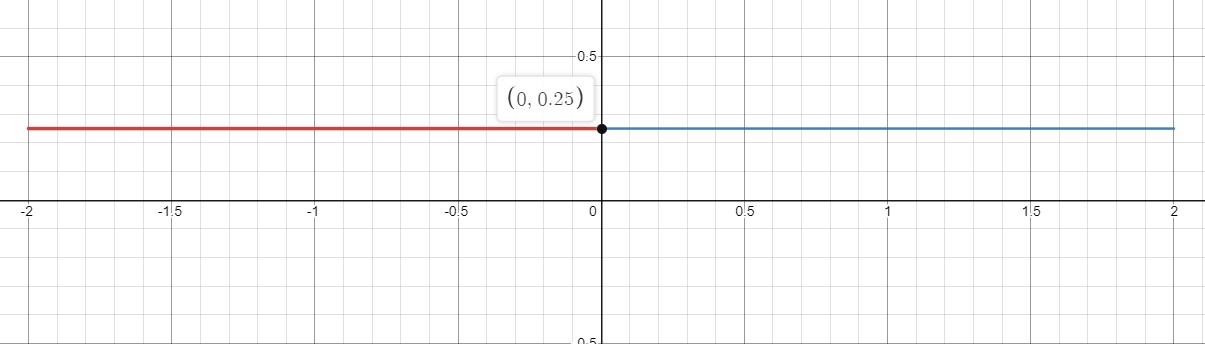
\includegraphics[width=\textwidth]{plot2}

\subsection*{(b)}
If the system is in idle mode, $M=0$, then $S=0$.
	So,
	$$ f_{Y|M} (y|0) = f_Z (y) $$

	So, $f_y$ takes the form of the distribution of $Z$, since there is only the ambient noise. The sketch is given by (in purple), \hfill \hfill \linebreak
	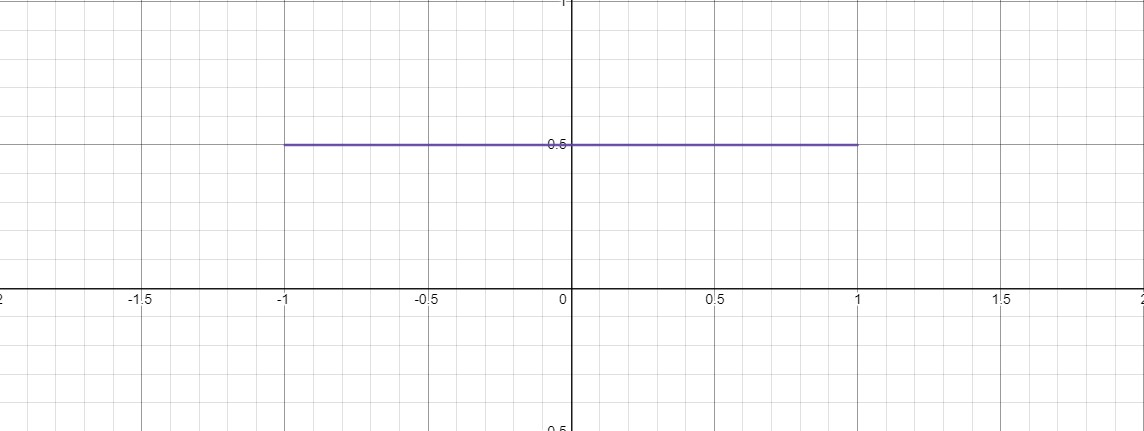
\includegraphics[width=\textwidth]{plot3}

\subsection*{(c)}
	We know that,
	$$ \hat M_{MAP} (x) = \arg \max_m P(m|y)  $$
	So, $ \hat M_{MAP} = 1$ if $f_{Y|M}(y|1) > f_{Y|M} (y|0)$, and $ \hat M_{MAP} = 0$ if $f_{Y|M}(y|1) < f_{Y|M} (y|0)$. From the sketch of $f_{Y|M}$ for both $M=1$ (red and blue) and $M=0$ (purple) given below, we can find the decision rule for optimal decoder $ \hat M_{MAP}$. \hfill \hfill
\linebreak
	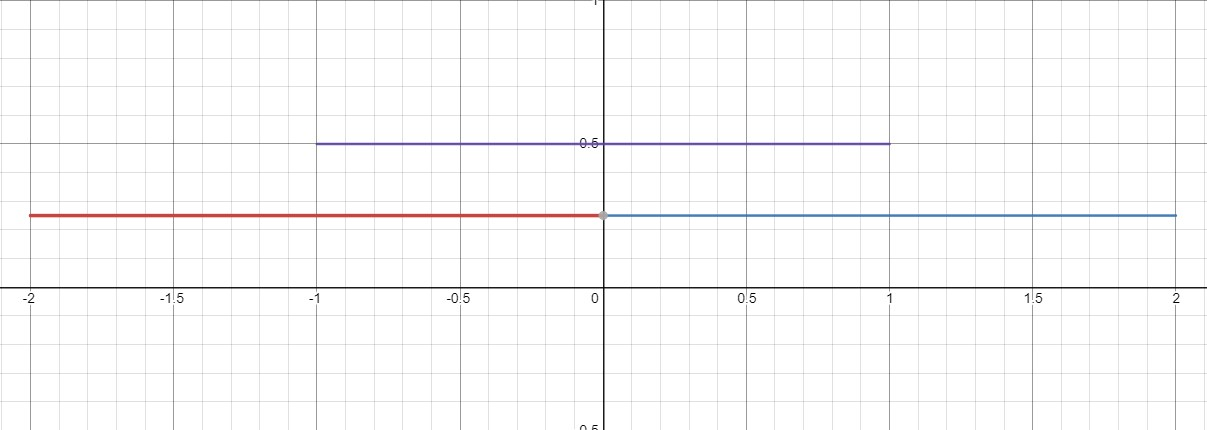
\includegraphics[width=\textwidth]{plot4}
\linebreak
\linebreak
	The optimal decoder $\hat{M}_{MAP} (y)$ is given by,
	$$ \hat{M}_{MAP} (y) = \begin{dcases}
		1 & y<-1 \\
		0 & -1<y<1 \\
		1 & y>1 \\
		\end{dcases}
	$$
\subsection*{(d)}
	The associated probability of error of our $\hat M_{MAP}$ is given by:
	$$ \begin{aligned}
		P(\hat M_{MAP} \neq M) &= P(\hat M_{MAP} = 1, M = 0)+P(\hat M_{MAP} = 0, M = 1) \\
		&= P(M=0, y<-1) + P(M=0, y>1) + P(M=1, -1<y<1) \\
		&= P(M=0) \cdot P(y<-1 | M=0) + P(M=0) \cdot P(y>1 | M=0) + P(M=1) \cdot P(-1<y<1 | M=1) \\
		&= \frac{1}{2} \cdot 0 + \frac{1}{2} \cdot 0 + \frac{1}{2} \cdot  \int_{-1}^{1} 0.25 \ dy \\
		&= 0 + 0 + \frac{1}{2} \cdot \left[ \frac{y}{4}\right]_{-1}^{1} \\
		&= \frac{1}{2} \cdot 0.5 \\
		&= 0.25 \\
	\end{aligned}
	$$

\section*{Problem 5}
	We know that,
	$$ X = \begin{dcases}
		1 & with\ probability\ \frac{1}{2} \\
		10 & with\ probability\ \frac{1}{2}
		\end{dcases}
	$$
	$$ \hat{X}_{MAP} = \arg \max_x P(x|y) $$
\linebreak
	
	For $X=1$,
	$$ \begin{aligned}
		P(X=1 | Y=y) &= \frac{P(Y=y|X=1)\cdot P(X=1)}{P(X=x)} \\
		 	&= \frac{P(Y=y|X=1)\cdot P(X=1)}{P(Y=y|X=1)\cdot P(X=1)+P(Y=y|X=2)\cdot P(X=2)} \\
			&= \frac{1^{y} \cdot e^{-1}}{1^{y} \cdot e^{-1}+10^{y} \cdot e^{-10}}
	\end{aligned}
	$$
\linebreak
	
	For $X=1$,
	$$ \begin{aligned}
		P(X=1 | Y=y) &= \frac{P(Y=y|X=1)\cdot P(X=1)}{P(X=x)} \\
		 	&= \frac{P(Y=y|X=1)\cdot P(X=1)}{P(Y=y|X=1)\cdot P(X=1)+P(Y=y|X=2)\cdot P(X=2)} \\
			&= \frac{10^{y} \cdot e^{-10}}{1^{y} \cdot e^{-1}+10^{y} \cdot e^{-10}}
	\end{aligned}
	$$
\linebreak

	To find the critical point $y*$.
	$$ \frac{1^{y*} \cdot e^{-1}}{1^{y*} \cdot e^{-1}+10^{y*} \cdot e^{-10}} = \frac{10^{y*} \cdot e^{-10}}{1^{y*} \cdot e^{-1}+10^{y*} \cdot e^{-10}} $$
	$$ \Rightarrow y* = \frac{9}{log(10} \approx 3.9 \approx 4 $$

	Now, if $y=3$, $P(X=1|Y=y) \approx 0.89$. So, our decision rule is given by,
	$$ \hat{X}_{MAP} = \begin{dcases}
		1, & y<4 \\
		10, & otherwise \\
		\end{dcases}
	$$

	So our $y*= 4 $.

	Now, the probability of error is given by,
	$$ \begin{aligned}
P(\hat{X}_{MAP} \neq X) &= P(X=10,Y<4) \cup P(X=1,Y>4) \\
		&= P(Y<4|X=10)\cdot P(X=10) +P(Y>4|X=1)\cdot P(X=1) \\
		&= P(X=10) \cdot \left[ \sum_{i=0}^{3} P(Y=i|X=10) \right] + P(X=1) \cdot \left[ 1- \sum_{i=0}^{3} P(Y=i|X=1) \right] \\
		&= \frac{1}{2} \cdot \left[ \sum_{i=0}^{3} \frac{10^{i} e^{-10}}{i!} \right] + \frac{1}{2} \cdot \left[ 1- \sum_{i=0}^{3} \frac{1^i e^{-1}}{i!} \right] \\
		&\approx \frac{1}{2} \left[ 0.01034+0.01899 \right] \\
		&= 0.014665 \\
	\end{aligned}
	$$

\section*{Problem 6}
	We know that $\Theta \sim$ Unif$[101,200]$ and given $\Theta$, $X \sim$ Unif$[1,\Theta]$. 
	$$ \hat\Theta_{MAP} = \arg \max_{\theta} P(\theta |x) $$

	Now, $$ \begin{aligned}
	P(\Theta = \theta | X=x ) &= \frac{P(X=x|\Theta = \theta) \cdot P(\Theta = \theta)}{P(X=x} & when\ x\ \in [1,\theta] \\
		&= \frac{\frac{1}{\theta - 1}\cdot \frac{1}{200-101 + 1}}{P(X=x)} & \\ 
		\end{aligned}
	$$
	We can see that $P(X=x)$ is independent of $\theta$, so we can maximize,
	$$ \frac{1}{\theta - 1} \cdot \frac{1}{100} $$
	
	For $\theta > 1$, the above function is monotonically decreasing. So we get two cases,
	$$ \hat{\Theta}_{MAP} = \begin{dcases}	
		101, &  x < 101 \\
		x, & x \in  [101, 200] \\
		\end{dcases}
	$$


\end{document}